
% DEFINE SOME HANDY SYMBOLS:
%\simlt and \simgt produce > and < signs with twiddle underneath
\def\spose#1{\hbox to 0pt{#1\hss}}
\def\simlt{\mathrel{\spose{\lower 3pt\hbox{$\mathchar"218$}}
     \raise 2.0pt\hbox{$\mathchar"13C$}}}
\def\simgt{\mathrel{\spose{\lower 3pt\hbox{$\mathchar"218$}}
     \raise 2.0pt\hbox{$\mathchar"13E$}}}
%\simpropto produces \propto with twiddle underneath
\def\simpropto{\mathrel{\spose{\lower 3pt\hbox{$\mathchar"218$}}
     \raise 2.0pt\hbox{$\propto$}}}
\def\tauc{\tau_\textrm{CMB}}

\newcommand{\acl}[1]{{\color{red} \textbf{[ACL:  #1]}}}

\documentclass[twocolumn,aps,prd,nofootinbib,showpacs]{revtex4-1}
\usepackage{amsmath,graphicx,bm,color}
\begin{document}
\title{Optical Depth from $21\,\textrm{cm}$}


\date{\today}



\pacs{95.75.-z,98.80.-k,95.75.Pq,98.80.Es}


\begin{abstract}

\end{abstract}

\maketitle

\section{Introduction}
\begin{itemize}
\item Reionization is not only an interesting epoch to study in its own right, but also because it's a nuisance for the CMB.  If we can understand reionization, we can predict $\tau_{CMB}$.  We can then send our prediction to our CMB friends so that they no longer have to marginalize over it.  In turn, that gives us better cosmological constraints on the other parameters.  This paper is timely because we have next-generation instruments (like HERA!) coming online.
\end{itemize}


\section{Tau Predictions}
\begin{itemize}
\item What does it take to predict tau? Emphasize the point that Jonathan made: it's the density-weighted ionization fraction that counts. So it's more complicated than just integrating an ionization history. Perhaps this would be a good place to add Jonathan's nice plots from global inside-out, outside-in, local... etc.?
\end{itemize}

Roughly speaking, we envision a multi-stage process for using $21\,\textrm{cm}$ measurements for constraining $\tauc$. First, qualitatively different models are distinguished from one another with coarse measurements of the power spectrum or even higher order statistics \acl{Cite Watkinson and Pritchard}. Having selected a single model out of many, one then uses precision power spectrum measurements to fix free parameters within the model. The correlated ionization and density fields of the model can then be predicted from simulations, and the optical depth estimated. This simulation-derived optical depth may, however, deviate from the ``true" value of $\tauc$ in our Universe because simulations depend on random realizations of density fields. If this ``simulation variance" on $\tauc$ is small enough to be tolerable, one may immediately feed the derived value of $\tauc$ into broader cosmological parameter estimations. On the other hand, if the simulation variance is large, it becomes necessary to directly measure the realization of $\tauc$ that represents our Universe. To do so, we propose using power spectrum measurements to restrict the space of possible reionization histories, enabling a principal component-based parameterization that can then be precisely constrained using a global signal measurement. Through the linearity arguments presented above \acl{Make sure these are included, or discuss them here}, these essentially constitute a direct measurement of the optical depth.

\subsection{Tau predictions from power spectrum measurements}
\begin{itemize}
\item Power spectrum measurements are a rather poor way of doing it, but they're the most promising short-term observable. So we're choosing to take a look at it, even though it's quite model dependent. It'll essentially require tying the measurements to simulations. We assume that large qualitative changes to reionization physics have already been ruled out in an earlier model selection step.
\item Talk about the models and why it's ok to ignore spin temperature (basically ionization frac is too low when spin temperature effects are important). But maybe we should quantify this a little.
\item Point out the interesting feature where the degeneracies in 21cm don't compromise our ability to predict tau.

Of course, no probe of reionization is perfect, and any practical measurement will come with its attendant errors and degeneracies. For example, in \acl{Cite Jonnie and Grieg \& Mesinger} it was shown that except in the extremely high signal-to-noise regime, fits to theoretical model parameters from $21\,\textrm{cm}$ power spectrum measurements are prone to strong degeneracies if performed at a single redshift. Multi-redshift observations break these degeneracies to a great extent, enabling for instance $\sim 10\%$ level constraints \acl{Check numbers} from upcoming instruments like HERA. However, some degeneracy will remain, as evidenced by the elliptical contours shown in Figure \ref{fig:21cmDegen_wTau}, which show some example $68\%$ and $95\%$ confidence regions on $T_\textrm{vir}$ and $\zeta$ constraints. These are derived from Fisher matrix forecasts assuming multi-redshift power spectrum measurements performed by HERA \acl{Specify a lot more what went into this calculation, especially regarding foregrounds}. There is clearly a degeneracy that persists between the two parameter.

\begin{figure}[!]
	\centering
	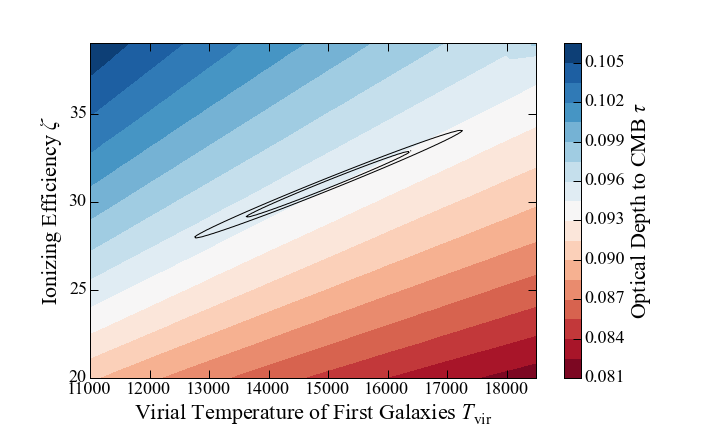
\includegraphics[width=0.5\textwidth]{figures/21cmDegen_wTau.png}
	\caption{asdf}
	\label{fig:21cmDegen_wTau}
\end{figure}

Fortunately, these residual degeneracies have relatively impact on one's ability to predict $\tau$. Performing a simulation of the ionization field for every point in the parameter space shown in Figure \label{fig:21cmDegen_wTau}, the relevant integral \acl{Reference the equation} can be evaluated to give predictions for $\tau$. The resulting solid color contours in Figure \label{fig:21cmDegen_wTau} are seen to be quite closely aligned to elliptical contours, suggesting that a very precise value for $\tau$ can be obtained from $21\,\textrm{cm}$ measurements even in the face of degeneracies.

\item Show $\tau$ predictions for both a WMAP-style redshift and a (probably lower tau) Planck redshift.
\item Talk about whether a bigger array does much better.
\end{itemize}
\subsection{Tau predictions from global signal measurements}
\begin{itemize}
\item Show that global signal measurements can get to precisely the quantity we need. But we need to limit the number of degrees of freedom in our fits in order for it to work.
\item Power spectrum measurements can help to provide a basis for global signal measurements. Show PCA modes for deviations from fiducial signal.

\begin{figure}[!]
	\centering
	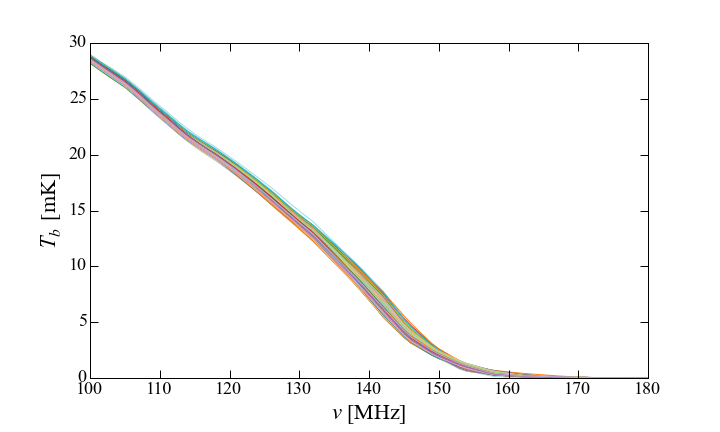
\includegraphics[width=0.5\textwidth]{figures/sampled_Tb_cutoff.png}
	\caption{asdf}
	\label{fig:sampled_Tb_cutoff}
\end{figure}

\begin{figure}[!]
	\centering
	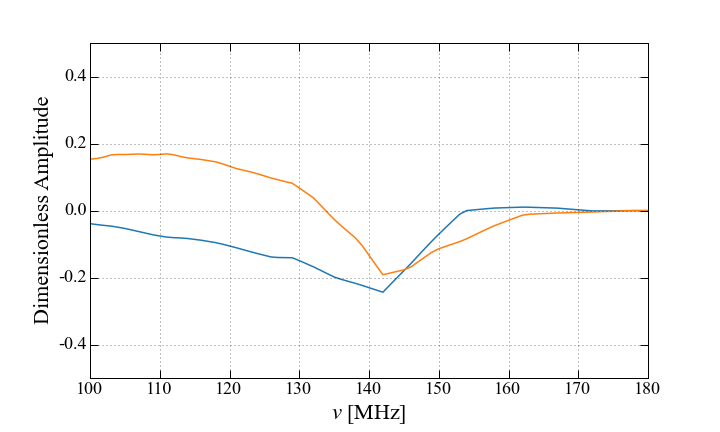
\includegraphics[width=0.5\textwidth]{figures/PCA_cutoff.png}
	\caption{asdf}
	\label{fig:PCA_cutoff}
\end{figure}


\begin{figure}[!]
	\centering
	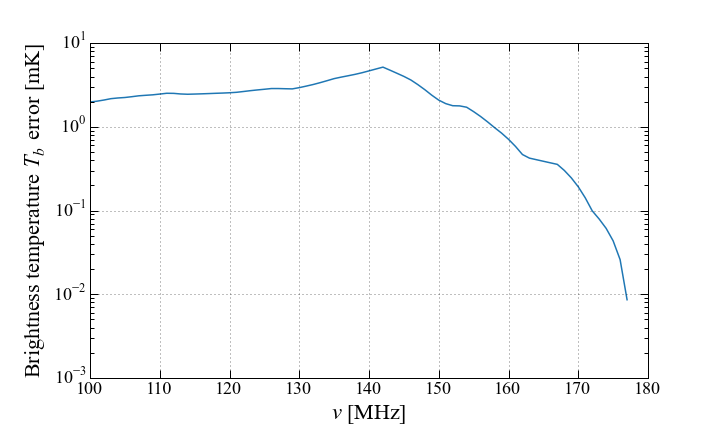
\includegraphics[width=0.5\textwidth]{figures/Tb_global_errors.png}
	\caption{asdf}
	\label{fig:Tb_global_errors}
\end{figure}

\item Some forecasts for constraining these deviation modes. Show different foreground subtraction scenarios.
\item Point out the fact that by making a direct measurement, we avoid the problem of cosmic variance, since we're essentially measuring ``our" tau, in our branch of the multiverse.
\end{itemize}
%\subsection{Tau predictions from imaging experiments}
%\item As far as predicting tau is concerned, an imaging experiment is just a very high signal-to-noise global signal experiment.
%\item However, one must be careful because an interferometer does not measure the zero-mode spatially. Need to rely on the assumption that at the relevant redshifts, we are in emission, so the brightness temperature is greater than or equal to zero. This lets us recover the zero-point.
%\item Perform thermal noise calculation.
%\item Give tau predictions
%\end{itemize}
\subsection{Summary of tau predictions}
\begin{itemize}
\item Provide a table summarizing values.
\end{itemize}

\section{Improvements in the CMB}
\subsection{Degeneracy breaking}
Highlight some specific examples.
\begin{itemize}
\item How might it be helpful to no longer have the $A_s$ and $\tau$ degeneracy?

\begin{figure}[!]
	\centering
	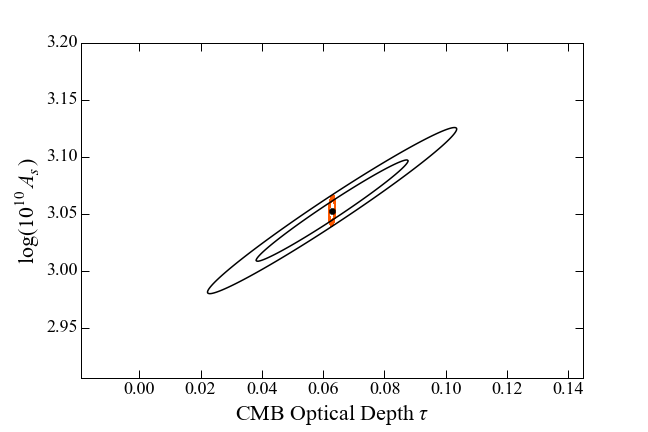
\includegraphics[width=0.5\textwidth]{figures/AsTau_w21cm.png}
	\caption{asdf}
	\label{fig:AsTau_w21cm}
\end{figure}

\item What about B-modes? Reionization bump predictions need $\tau$, so consistency tests are helped by 21cm. Also discuss Mortonson \& Hu (2008) and how inflationary parameters are biased if reionization not modeled correctly.
\end{itemize}

\section{Predictions for $x_{HI}$}
Mention how even thought it's not $x_{HI}$ that's directly relevant for $\tau$, the same measurements mentioned earlier might provide a way to probe the ionized fraction (particularly the power spectrum measurements).
\begin{itemize}
\item Show some projections for $x_{HI}$.
\item Talk about how this can be very complementary to optical/IR measurements.
\end{itemize}

\section{Conclusions}
Summarize our main points.

\section*{Acknowledgments}


\bibliography{21cmTau}


\end{document}
